\documentclass{article}

\usepackage{fancyhdr}
\usepackage{extramarks}
\usepackage{amsmath}
\usepackage{amsthm}
\usepackage{amsfonts}
\usepackage{tikz}
\usepackage[plain]{algorithm}
\usepackage{algpseudocode}
\usepackage{enumitem}
\usepackage{minted}
\usepackage{verbatim}
\usepackage{amssymb}
\usepackage{graphicx}
\usepackage[superscript,biblabel]{cite}
\usepackage{url}
%\usepackage{showframe}
\usepackage{import}

\usepackage{pstricks}
\usepackage{pst-plot}
\usepackage{pst-3dplot}
\usepackage{pst-tools}
\usepackage{caption}

\graphicspath{ {images/} }

\usetikzlibrary{automata,positioning}

%
% Basic Document Settings
%

\topmargin=-0.45in
\evensidemargin=0in
\oddsidemargin=0in
\textwidth=6.5in
\textheight=9.0in
\headsep=0.25in

\linespread{1.1}

\pagestyle{fancy}
%\lhead{\firstxmark}
%\chead{\hmwkTitle}
\lhead{\hmwkTitle}
\rhead{\hmwkAuthorName}
\lfoot{\lastxmark}
\cfoot{\thepage}

\renewcommand\headrulewidth{0.4pt}
\renewcommand\footrulewidth{0.4pt}

\setlength\parindent{0pt}

%
% Create Problem Sections
%

\newcommand{\enterProblemHeader}[1]{
    \nobreak\extramarks{}{Problem \arabic{#1} continued on next page\ldots}\nobreak{}
    \nobreak\extramarks{Problem \arabic{#1} (continued)}{Problem \arabic{#1} continued on next page\ldots}\nobreak{}
}

\newcommand{\exitProblemHeader}[1]{
    \nobreak\extramarks{Problem \arabic{#1} (continued)}{Problem \arabic{#1} continued on next page\ldots}\nobreak{}
    \stepcounter{#1}
    \nobreak\extramarks{Problem \arabic{#1}}{}\nobreak{}
}

\setcounter{secnumdepth}{0}
\newcounter{partCounter}
\newcounter{homeworkProblemCounter}
\setcounter{homeworkProblemCounter}{1}
\nobreak\extramarks{Problem \arabic{homeworkProblemCounter}}{}\nobreak{}

%
% Homework Problem Environment
%
% This environment takes an optional argument. When given, it will adjust the
% problem counter. This is useful for when the problems given for your
% assignment aren't sequential. See the last 3 problems of this template for an
% example.
%
\newenvironment{homeworkProblem}[1][-1]{
    \ifnum#1>0
        \setcounter{homeworkProblemCounter}{#1}
    \fi
    \section{Problem \arabic{homeworkProblemCounter}}
    \setcounter{partCounter}{1}
    \enterProblemHeader{homeworkProblemCounter}
}{
    \exitProblemHeader{homeworkProblemCounter}
}

%
% Homework Details
%   - Title
%   - Due date
%   - Class
%   - Instructor
%   - Author
%

\newcommand{\hmwkTitle}{Assignment 1}
\newcommand{\hmwkDueDate}{Feb 27, 2018 11:55 pm}
\newcommand{\hmwkClass}{CS-GY 6643 Computer Vision}
\newcommand{\hmwkClassInstructor}{Guido Gerig}
\newcommand{\hmwkAuthorName}{\textbf{Tianyu Wang}}

%
% Title Page
%

\title{
    \vspace{2in}
    \textmd{\textbf{\hmwkClass\\\hmwkTitle}}\\
    \normalsize\vspace{0.1in}\small{Due\ on\ \hmwkDueDate}\\
    \vspace{0.1in}\large{\textit{Professor \hmwkClassInstructor}}
    \vspace{3in}
}

\author{\hmwkAuthorName}
\date{}

\renewcommand{\part}[1]{\textbf{\large Part \Alph{partCounter}}\stepcounter{partCounter}\\}

%
% Various Helper Commands
%

% Useful for algorithms
\newcommand{\alg}[1]{\textsc{\bfseries \footnotesize #1}}

% For derivatives
\newcommand{\deriv}[1]{\frac{\mathrm{d}}{\mathrm{d}x} (#1)}

% For partial derivatives
\newcommand{\pderiv}[2]{\frac{\partial}{\partial #1} (#2)}

% Integral dx
\newcommand{\dx}{\mathrm{d}x}

% Alias for the Solution section header
\newcommand{\solution}{\textbf{\large Solution}}

% Probability commands: Expectation, Variance, Covariance, Bias
\newcommand{\E}{\mathrm{E}}
\newcommand{\Var}{\mathrm{Var}}
\newcommand{\Cov}{\mathrm{Cov}}
\newcommand{\Bias}{\mathrm{Bias}}

\newcommand{\forceindent}{\leavevmode{\parindent=2em\indent}}
\newcommand\Item[1][]{%
  \ifx\relax#1\relax  \item \else \item[#1] \fi
  \abovedisplayskip=0pt\abovedisplayshortskip=0pt~\vspace*{-\baselineskip}}

\begin{document}
\maketitle
\pagebreak

\subsection{Part A - Theoretical Questions}
\begin{enumerate}[label=A\arabic*)]
% %[label=(\Alph*)]
% %[label=(\roman*)]
% 	\item \import{/}{a.tex}
% 	\item \import{/}{b.tex}
	\item Image formation 
		\\
		\\
		A professional full-frame digital camera uses an image size of 36mm x 36mm and standard focal length of 50mm. Let us say that the square sensor provide 16 megapixels. Now you buy smartphone with a 16 megapixel sensor (assuming a square image too), but given a focal length of 4mm so that the phone fits into your pocket.
		\begin{itemize}
			\item Using the pinhole camera projection equation, calculate the size of the light-sensitive image sensor of your smart-phone. Calculate the ratio of this size relative to the professional camera sensor size.
			\item Calculate the size of a sensor pixel element for the professional and your smart-phone cameras. Provide a short discussion of eventual advantages/disadvantages of your resulting measures, and reasons why some professionals or amateurs favor more expensive large cameras.
			\item Calculate the storage requirement assuming storage of raw images with color RGB channels, for both cameras.	
		\end{itemize}

		
	\item Connectivity foreground/background 
		\\
		\\
		One solution to digitization paradoxes is to mix connectivities. Using 8-neighborhood for foreground and 4-neighborhood for background, examine the paradoxes shown in the book (Fig. 2.7). Discuss the number of components of fore- versus background given this choice. Also discuss the \#of components when either using 4-n (and also 8-n) for both fore- and background, and when reversing the notion and using 8-n for background and 4-n for foreground. You can discuss in words and also include sketches of your thoughts to this section.
		\begin{figure}[h!]
			\centering
			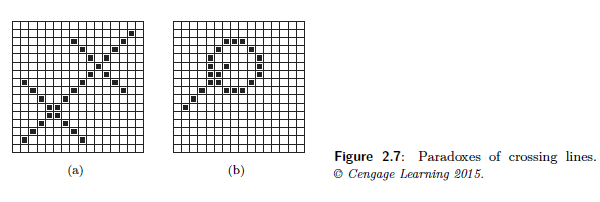
\includegraphics[width=\linewidth-20em]{img-1.png}
		\end{figure}
	\item Histogram equalization
		\\
		\\
		Remember the main goal of histogram equalization to result in a uniform intensity distribution (histogram). Below you see the images from the book referring to image equalization. Explain why the histogram of a discrete image is not flat after histogram equalization. (Hint: You may first work on the practical part to get a closer insight).
		\begin{figure}[h!]
			\begin{minipage}{0.48\textwidth}
				\centering
				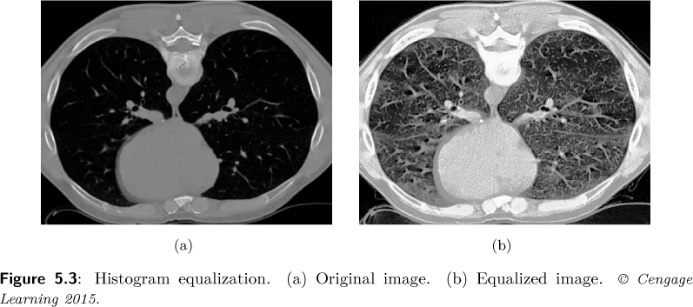
\includegraphics[width=.9\linewidth]{img-2.png}
			\end{minipage}
			\hfill
			\begin{minipage}{0.48\textwidth}
				\centering
				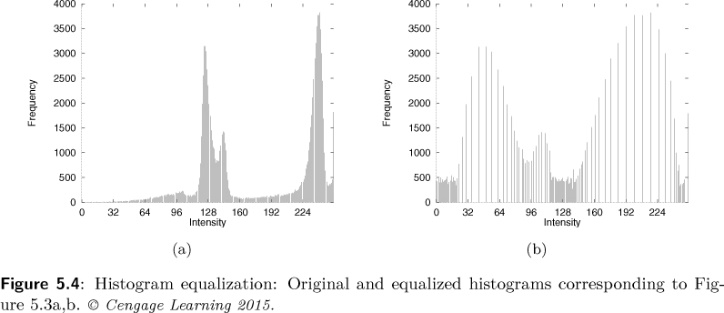
\includegraphics[width=.9\linewidth]{img-3.png}
			\end{minipage}
		\end{figure}
\end{enumerate}

\pagebreak

\subsection{Answers}
\begin{enumerate}[label=A\arabic*)]
	\item Image formation 
		\begin{itemize}
			\item According to the projection equation, we have:
				\begin{align*}
					\frac{Length\:of\:the\:edge}{Focal\:length} &= \frac{36\:mm}{50\:mm} 
					\\ &= \frac{x}{4\:mm}
					\\ \Rightarrow\:x\:=\:2.88\:mm
				\end{align*}
				So the size of the light-sensitive image sensor of your smart-phone should be $2.88\:mm \times 2.88\:mm$. And the ratio should be
				\begin{align*}
					ratio\:=\:\frac{4\:mm}{50\:mm}\:=\:\frac{2}{25}
				\end{align*}
			 \item The square sensor provides 16 megapixels for a square image. So the size of the square image should be $4000 \times 4000$.
				\begin{enumerate}[label=(\roman*)]
					\item The size of a sensor pixel element for the professional digital camera:
						\begin{align*}
							Length\:of\:the\:edge\:of\:a\:pixel\:element\:&=\:\frac{36\:mm}{4000}\:=\:0.009\:mm\:=\:9\:\mu m \\
							Size\:of\:a\:pixel\:element\:&=\:(Length\:of\:the\:edge\:of\:a\:pixel\:element)^2 \\
							&=81\:\mu m^2 \\
						\end{align*}
					\item The size of a sensor pixel element for the smart-phone camera:
						\begin{align*}
							Length\:of\:the\:edge\:of\:a\:pixel\:element\:&=\:\frac{2.88\:mm}{4000}\:=\:0.00072\:mm\:=\:0.72\:\mu m \\
							Size\:of\:a\:pixel\:element\:&=\:(Length\:of\:the\:edge\:of\:a\:pixel\:element)^2 \\
							&=0.5184\:\mu m^2 \\
						\end{align*}
					\item 
						\begin{tabular}{ | r | c | c |}
						\hline
						 & \textbf{Advantages} & \textbf{Disadvantages} \\
						\hline
						Professional digital camera & \textbf{Quality}: high & \textbf{Size}: large \\
						Smart-phone & \textbf{Size}: small & \textbf{Quality}: low \\
						\hline
						\end{tabular}
						\\
						\\
						(p.s: ‘size’ means 'size of a pixel element', not the real 'image size', which is the same for both.)
					\item \textbf{Conclusion}: Large professional digital cameras have better image quality. They have larger image element size, which means that the raster in a camera can absorb more light than smart-phone. Although cameras are much heavier and larger than a smart-phone, they can take better pictures and provide more details in a photo.
				\end{enumerate}
				\item The size of image taken by a digital camera or smart-phone is same with each other. So for one raw image:
					\begin{align*}
						Storage\:of\:raw\:image\:&=\:Pixels\:in\:this\:photo \times Storage\:of\:per\:pixel\\
						&= (4000 \times 4000) \times (8\:bits \times 3\:channels) \\
						&= 48,000,000\:bytes \approx 48\:\text{MB}
					\end{align*}
		\end{itemize}
		\pagebreak
	\item Connectivity foreground/background
\begin{enumerate}[label=(\alph*)]
			\item
				\begin{enumerate}[label=\arabic*)]
					\item $D_8$ for foreground and $D_4$ for background \\
						\forceindent Number of components in foreground: 1 \\
						\forceindent Number of components in background: 1
					\item $D_4$ for foreground and $D_4$ for background \\
						\forceindent Number of components in foreground: 25 \\
						\forceindent Number of components in background: 1
					\item $D_8$ for foreground and $D_8$ for background \\
						\forceindent Number of components in foreground: 1 \\
						\forceindent Number of components in background: 1
					\item $D_4$ for foreground and $D_8$ for background \\
\forceindent Number of components in foreground: 25 \\
						\forceindent Number of components in background: 1
				\end{enumerate}
				\begin{tabular}{ | r | c | c |}
					\hline
					 & $D_4$ & $D_8$ \\
					\hline
					\textbf{\# of components in foreground} & 25 & 1 \\
					\textbf{\# of components in background} & 1 & 1 \\
					\hline
				\end{tabular}
			\item
				\begin{enumerate}[label=\arabic*)]
					\item $D_8$ for foreground and $D_4$ for background \\
						\forceindent Number of components in foreground: 1 \\
						\forceindent Number of components in background: 2
					\item $D_4$ for foreground and $D_4$ for background \\
						\forceindent Number of components in foreground: 11 \\
						\forceindent Number of components in background: 2
					\item $D_8$ for foreground and $D_8$ for background \\
						\forceindent Number of components in foreground: 1 \\
						\forceindent Number of components in background: 1
					\item $D_4$ for foreground and $D_8$ for background \\
\forceindent Number of components in foreground: 11 \\
						\forceindent Number of components in background: 1
				\end{enumerate}
				\begin{tabular}{ | r | c | c |}
					\hline
					 & $D_4$ & $D_8$ \\
					\hline
					\textbf{\# of components in foreground} & 11 & 2 \\
					\textbf{\# of components in background} & 1 & 1 \\
					\hline
				\end{tabular}
			\item \textbf{Thoughts}:
				\begin{itemize}
					\item \textbf{Foreground}: First, most of the lines/circles are not perfectly vertically/horizontally straight, or we can say, pixels are at the same line. So if we use $D_{4}$ to count the connected components in a line, we may wrongly separate these pixels into different parts. Furthermore, when we come across the situation where two lines are crossed with half pixels (see Figure 1), pixels inside of the purple square are counted into the same connected component. Therefore $D_{8}$ is better to be used to count the number of connected components in foreground.
%					\begin{minipage}{\linewidth}
%			            \centering
%			            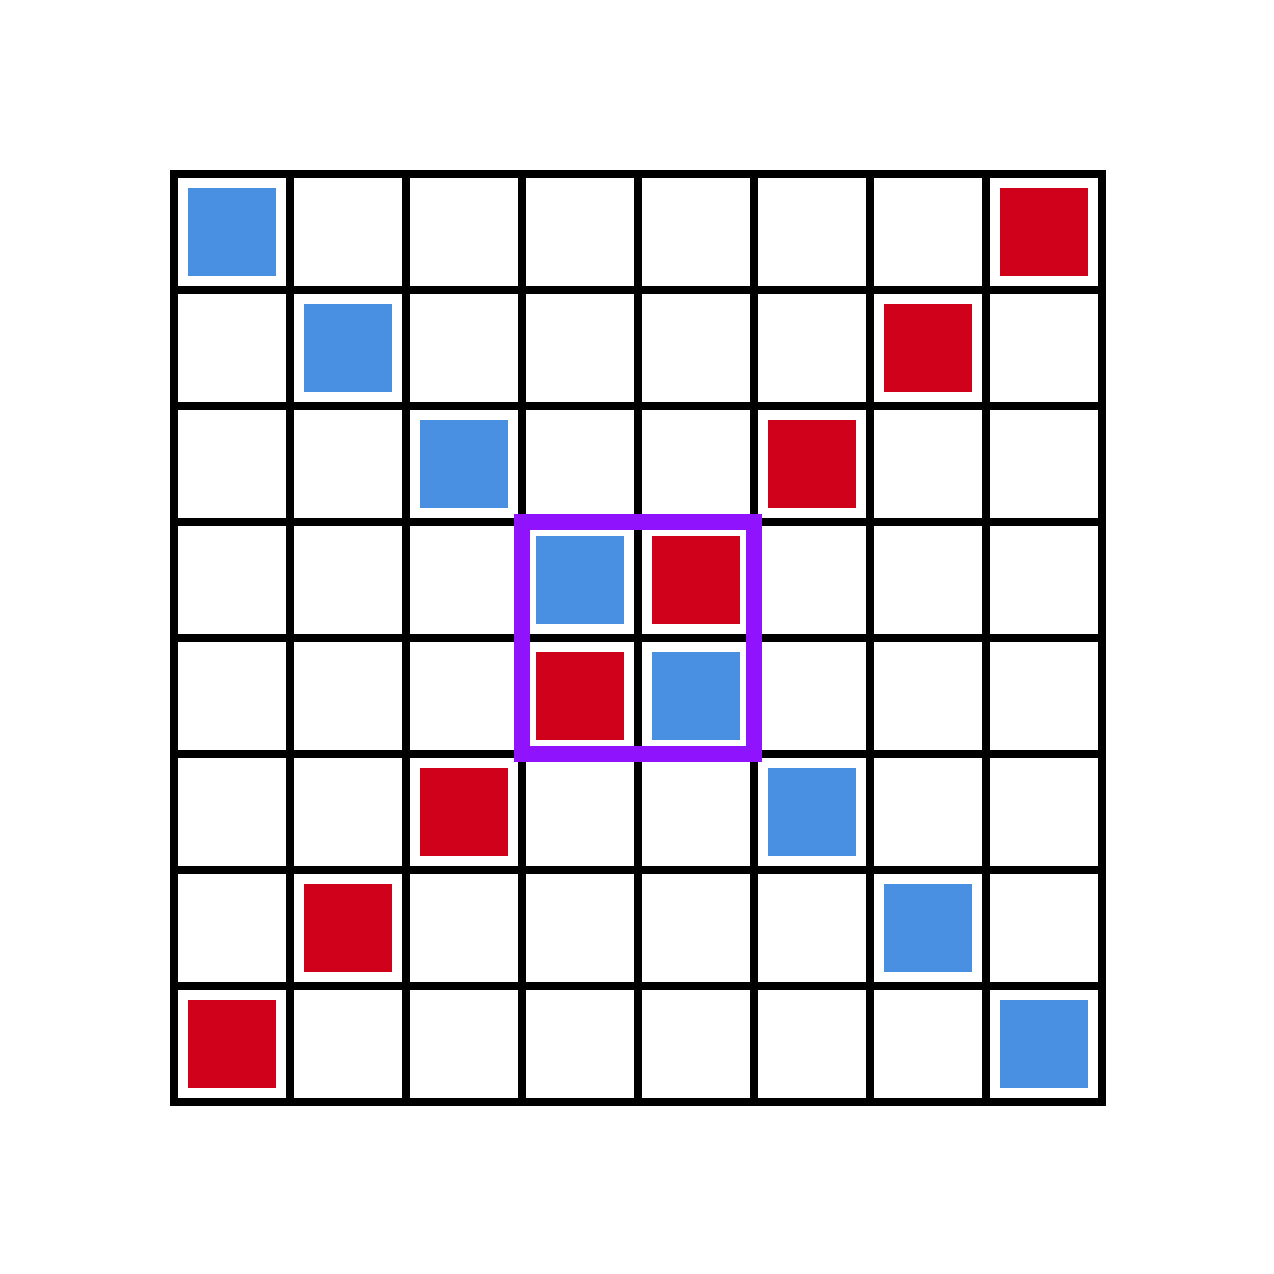
\includegraphics[width=\linewidth/2-10em]{img-4.jpg}
%			            \captionof{figure}{Two lines cross with each other}
%			        \end{minipage}
					\item \textbf{Background}: There's no circle in Figure 2.7(a) that can divide the background into 2 parts (using $D_{4}$). But in Figure 2.7(b), we can see that the circle divides the plane into 2 different parts. And if we use $D_{8}$ to calculate connected components, the area inside of the circle would be connected with the outside one. So we usually choose $D_{4}$ to count the number of connected components in background.
				\end{itemize}
				\begin{figure}[h!]
		            \centering
		            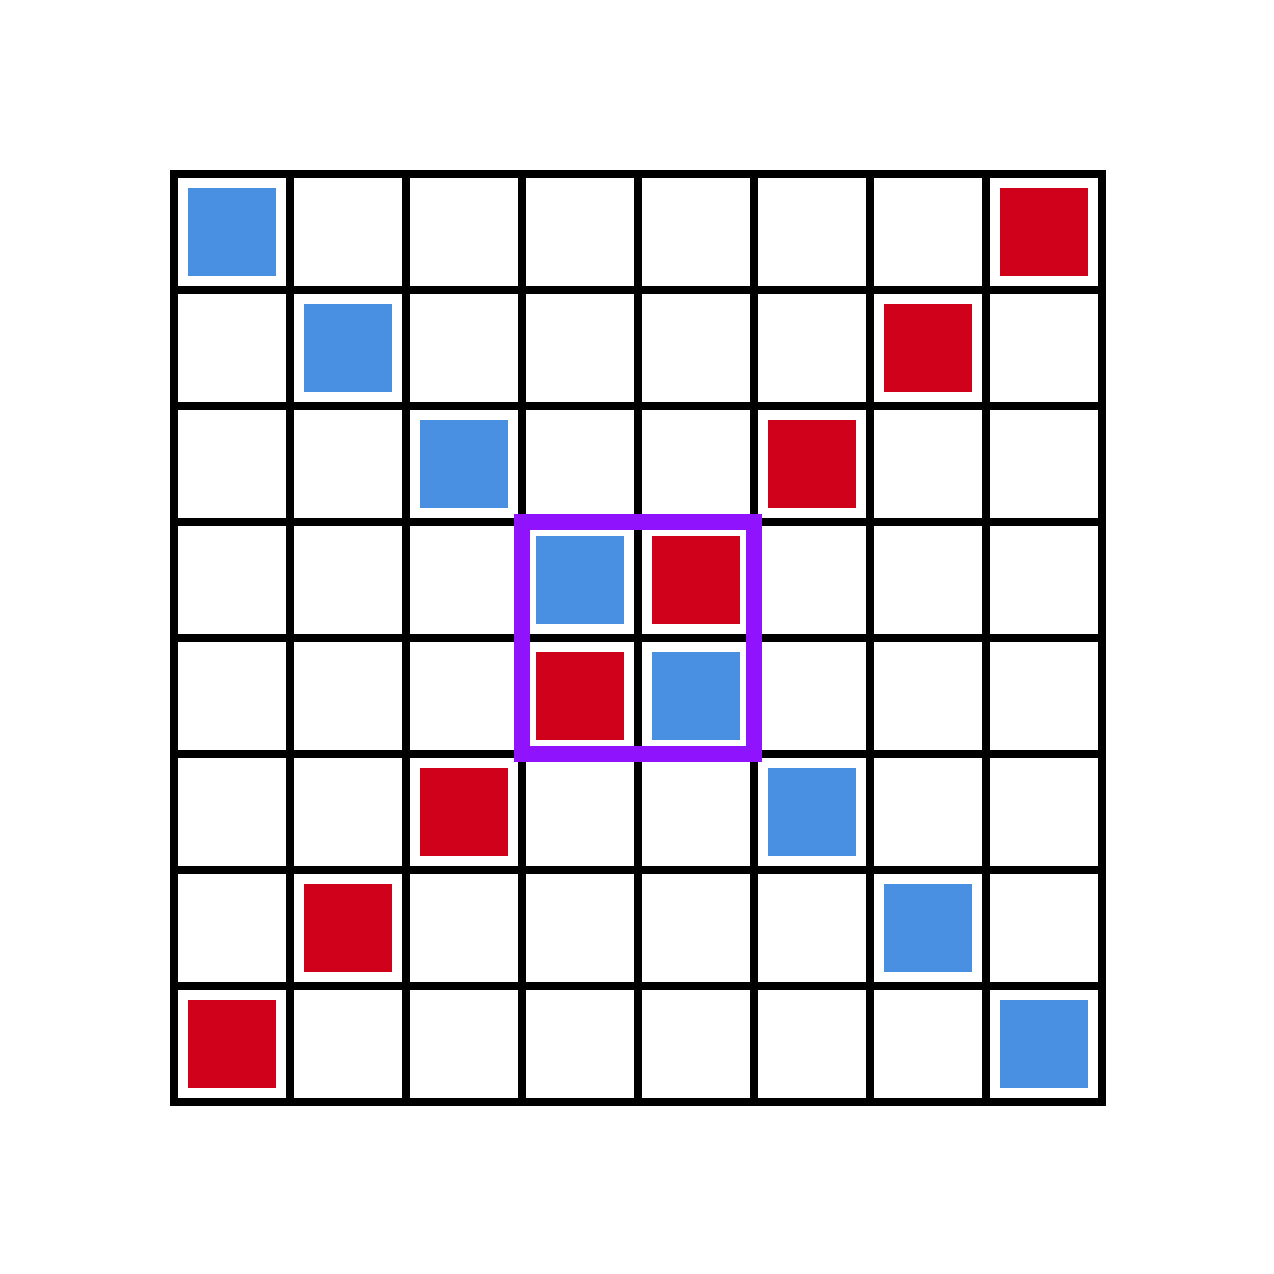
\includegraphics[width=\linewidth/3]{img-4.jpg}
		            \captionsetup{justification=centering}
		            \captionof{figure}{Two lines cross with each other}
		        \end{figure}
		\end{enumerate} 
	\pagebreak
	\item Histogram equalization
		\\
		\\
		There are mainly two reasons that would cause this problem:
		\begin{enumerate}[label=\arabic*)]
			\item No values are mapped into some particular values of the new equalized histogram (the black dots in Figure 2(a)).
			\item Different values are mapped into the same value of the new equalized histogram (the white dot in Figure 2(b)).
		\end{enumerate}
		\begin{figure}[h!]
            \centering
            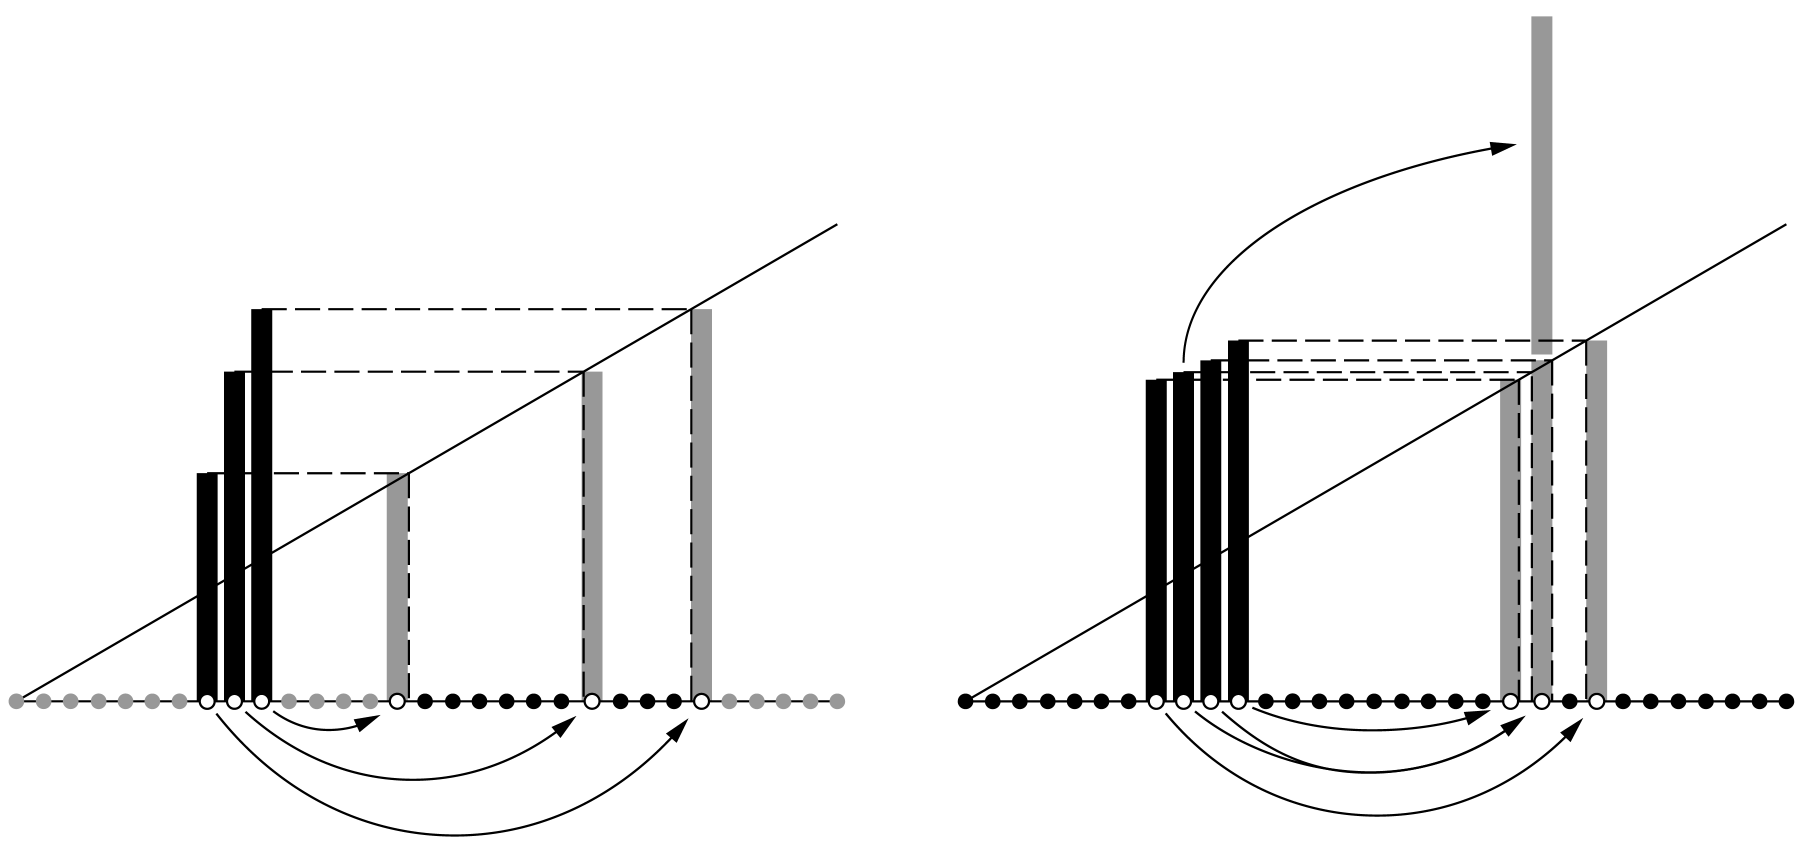
\includegraphics[width=\linewidth]{img-5.png}
            \captionsetup{justification=centering}
            \captionof{figure}{(a) no values are mapped into the specific value \\ (b) different values are mapped into the same value}
        \end{figure}
        Therefore, in the equalized histogram/pdf, we can see that there would be some peak values and also with some empty values. \\
        
        (Image Reference: \texttt{http://geomatica.como.polimi.it/corsi/rs\_ia/02\_Histogram\_manipulation.pdf})
\end{enumerate}
\pagebreak

\subsection{Part B - Practical Programming Assignments}
\begin{enumerate}[label=B\arabic*)]
	\item Compute a Histogram and CDF 
		\\
		\\
		Write code that reads a 2D image as input and returns a 1D array of the relative frequencies of occurrence of greylevels in your image. Provide a choice for quantizing a binning of the greylevels into n quantized bins between 0 and the maximum value (please remember that for an 8bit image, this is the range 0 … 255 for the range 0 … L-1).
		\begin{itemize}
			\item Calculate the histogram of an image of your choice, please note that a color image first needs to be converted into black-and-white.
			\item Normalize the histogram by the image size to present a probability density function (pdf), plot the pdf.
			\item Calculate the cumulative distribution function CDF from your pdf and plot the function.
			\item Creatively experiment with a second image that may show different structures.
			\item Write a short report that shows the original images, and the corresponding pdf and CDF plots. Provide a short discussion if the shape of the histograms that may reflect some of the visible properties of the image, and discuss differences between results from the two images.
		\end{itemize}

		
	\item Histogram Equalization 
		\\
		\\
		Use the histogram code as developed above, and provide an additional function for histogram equalization.
		\begin{itemize}
			\item Follow instructions as in the book and course notes to calculate the histogram, pdf, CDF and then a binning of the frequency axis into n bins that determines the mapping of intensities to form a uniform distribution.
			\item Apply your histogram equalization code to the images used before. Calculate and plot the new histogram after equalization.
			\item Add an additional section to the report by showing images, pdf’s and CDF’s before/after equalization. Briefly discuss what you see in the histogram equalized images and the corresponding plots of pdf’s and CDF’s.
		\end{itemize}
		
	\item Histogram Matching
		\\
		\\
		Following the course notes, develop code that maps intensity values of a preferably bad image into intensity distribution of a good looking image.
		\begin{itemize}
			\item Select an image with somewhat poor contrast or visibility of structures. Select a second image which looks good.
			\item Calculate histograms, pdf’s, CDF’s of both images. Follow course instructions to map the intensity distributions of the first image into those of the second image (histogram matching).
			\item Add a section to the report that shows original images and plots of pdf’s and CDF’s. Then show the results of the adjusted first image, and its pdf and CDF’s.
			\item Provide a short discussion of what you see and if the procedure resulted in the anticipated result.
		\end{itemize}		
\end{enumerate}

\pagebreak

\subsection{Report}
Before starting our project, we have to set up environment: I choose Python 3 and OpenCV-Python. You can use Jupyter or Google Colab to open my \texttt{.ipynb} file. I've also provided an online version (https://goo.gl/Bp3yYw) of this assignment for running.

\begin{enumerate}[label=B\arabic*)]
	\item Compute a Histogram and CDF 
		\\
		\\
		In this part, I picked up two images.
		\begin{enumerate}[label=\arabic*)]
			\item The \textit{Popeyes\textsuperscript{\tiny\textregistered} Fried Chicken} image %taken by myself:
				\begin{figure}[h!]
				\begin{minipage}{0.48\textwidth}
					\centering
					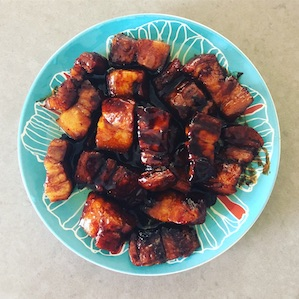
\includegraphics[width=20em]{Chicken/Original.jpg}
				\end{minipage}
				\hfill
				\begin{minipage}{0.48\textwidth}
					\centering
					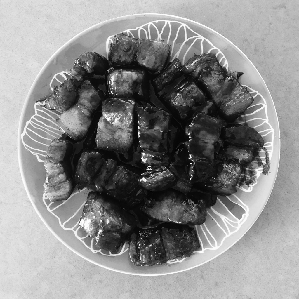
\includegraphics[width=20em]{Chicken/Gray.png}
				\end{minipage}
		\end{figure}

		\end{enumerate}
%		an image from OpenCV website to show its histogram and CDF.
		
	\item Histogram Equalization 
				
	\item Histogram Matching
		
\end{enumerate}


\end{document}
 